\chapter{Uživatelské rozhraní}\label{chap:UI}

Předchozí kapitola~\ref{chap:AppImplemetation} se zabývala převážně funkčností aplikace. V této kapitole se chci zaměřit na to, jak vypadá uživatelské rozhraní. Kapitola bude rozdělena do několika podkapitol, kdy každá z~nich se bude věnovat jedné stránce a tomu, co stránka obsahuje a jak se případně ovládá. 

\section{Spuštění aplikace}

Jelikož se jedná o webovou aplikace, tak k jejímu spuštění je potřeba webový prohlížeč, např. Mozilla Firefox, ve kterém bylo i aplikace testována. Samotné spuštění je již pak jednoduché --- stačí ve~Vámi zvoleném prohlížeči otevřít soubor \texttt{./dist/index.html}

\section{Hlavní stránka}

Když si uživatel zobrazí webovou stránku s aplikací, tak první, co uvidí, je hlavní nabídka. Ta je velice jednoduchá, protože obsahuje pouze nadpis a tři tlačítka vycentrované na středu stránky, Obrázek~\ref{fig:UIMainPage}. Každé z těchto tlačítek přepne uživatele na stránky, které budou popsané v dalších podkapitolách:
\begin{itemize}
    \item Tlačítko \texttt{New} --- Stránka pro tvorbu zásobníkového automatu, podkapitola~\ref{sec:PDABuilder}
    \item Tlačítko \texttt{Upload} --- Formulář pro nahrávání zásobníkových automatů, podkapitola~\ref{sec:UploadForm}
    \item Tlačítko \texttt{Saved} --- Výpis úložiště, podkapitola~\ref{sec:SimulatorPage}
\end{itemize}

\begin{figure}[h]
    \centering
    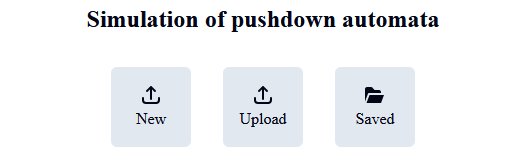
\includegraphics[width=0.8\textwidth]{Figures/PrntScrn_UI_MainMenu.png}
    \caption{Hlavní stránka}\label{fig:UIMainPage}
\end{figure}

\section{Stránka pro tvorbu zásobníkového automatu}\label{sec:PDABuilder}

Po kliknutí na tlačítko \texttt{new} v hlavní nabídce se otevře stránka pro tvorbu zásobníkového automatu. Tato stránka se skládá z několika formulářů a HTML input prvků. 

Jako první je textové pole pro specifikaci názvu automatu. Tento název se pak zobrazuje ve~výpisu automatů z úložiště. Dále následuje formulář pro přidávání stavů. Stavy se přidávají po jednom a jejich délka není omezená. Dále následují formuláře pro definování vstupní a zásobníkové abecedy. Symboly se opět přidávají po jednom a jejich délka je omezena na jeden znak. Vstupní pole pro~název a formulář pro přidávaní stavů lze vidět na Obrázku~\ref{fig:BuilderPart1} včetně chybové hlášky.

\begin{figure}[h]
    \centering
    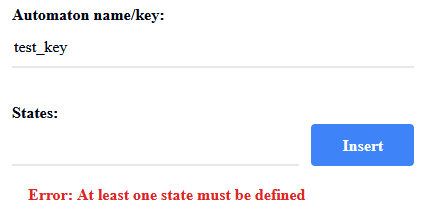
\includegraphics[width=0.5\textwidth]{Figures/PrntScrn_UI_BuilderPart1.png}
    \caption{Název a formulář pro přidávání stavů}\label{fig:BuilderPart1}
\end{figure}

Po těchto třech formulářích následují dva seznamy pro výběr počátečního stavu a počátečního zásobníkového symbolu. Dále následuje část pro určení, zda zásobníkový automat bude přijímat prázdným zásobníkem nebo přijímací stavy. To závisí na tom, zda uživatel zaškrtne zaškrtávacího pole. Pokud zůstane nezaškrtnuté, musí uživatel vybrat alespoň jeden ze stavů níže jako přijímací. Seznam počátečních zásobníkových symbolů a zaškrtávací pole je na Obrázku~\ref{fig:BuilderPart2}.

\begin{figure}[h]
    \centering
    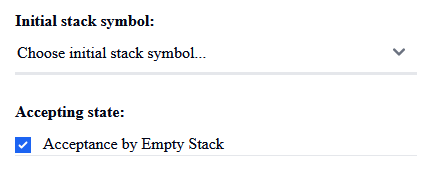
\includegraphics[width=0.5\textwidth]{Figures/PrntScrn_UI_BuilderPart2.png}
    \caption{Seznam počátečních zásobníkových symbolů a zaškrtávací pole pro určení typu zásobníkového automatu}\label{fig:BuilderPart2}
\end{figure}

Poslední část pak slouží k definování přechodů přechodové funkce. Její funkce již byla popsána v podkapitole~\ref{sec:PDABuilderImplementation}. Jak tato část vypadá lze vidět na Obrázku~\ref{fig:FilledTransition}. Pak již následují jen tlačítka na~navrácení na~hlavní stránku a uložené zásobníkového automatu.

\section{Formulář pro nahrávání zásobníkových automatů}\label{sec:UploadForm}

Druhým tlačítkem v hlavní nabídce se uživatel dostane na stránku s formulářem, který slouží k~nahrání zásobníkového automatu ze souboru. Formulář, Obrázek~\ref{fig:UploadForm}, je složen ze dvou částí. První je textové pole pro pojmenování automatu. Toto pole se používá jako klíč pro úložiště a zároveň se zobrazuje ve výpisu automatů. Pokud je klíč již použitý pro jiný automat, je při odeslání formuláře uživatel dotázán, zda chce automat s tímto klíčem přepsat. Druhé pole pak slouží pro nahrání souboru typu JSON, který obsahuje definici zásobníkového automatu. Při odeslání formuláře se nejprve ze souboru vytvoří instance třídy \texttt{PushdownAutomata} a následně se provede kontrola. Pokud automat nemohl být vytvořen kvůli neodpovídající struktuře nebo obsahuje chyby, je na to uživatel upozorněn společně s výpisem chyb, Obrázek~\ref{fig:PDACheckErrors}.

\begin{figure}[h]
    \centering
    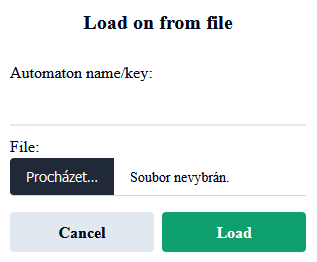
\includegraphics[width=0.45\textwidth]{Figures/PrntScrn_UI_Upload.png}
    \caption{Formulář pro nahrání zásobníkového automatu ze souboru}\label{fig:UploadForm}
\end{figure}

\section{Výpis úložiště}\label{sec:StoragePage}

Třetím tlačítkem v hlavní nabídce si uživatel může zobrazit seznam všech automatů, které jsou uložené v úložišti. Vzhled této stránky je na Obrázku~\ref{fig:Storage}. Nad samotnou tabulkou je nadpis a~tlačítko pro návrat do hlavní nabídky. Samotná tabulka pak má 6 sloupců a každý řádek odpovídá jednomu automatu v úložišti.

První sloupec obsahuje název automatu, dalších 5 sloupců pak obsahuje tlačítka. První tlačítko zobrazí stránku, na které je tabulka s informacemi o automatu. Druhé tlačítko přepne uživatele na~stránku pro tvorbu zásobníkového automatu, kde může uživatel automat zeditovat. Třetí tlačítko přepne uživatel na stránku simulátoru, která je popsána v podkapitole~\ref{sec:SimulatorPage}, a nastaví tam konkrétní zásobníkový automat. Čtvrté tlačítko pak slouží pro stažení automatu jako soubor typu JSON.\ Poslední tlačítko pak slouží pro vymazání automatu z úložiště.

\begin{figure}[h]
    \centering
    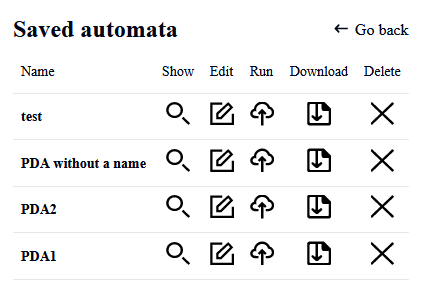
\includegraphics[width=0.5\textwidth]{Figures/PrntScrn_UI_Storage.png}
    \caption{Výpis automatů v úložišti}\label{fig:Storage}
\end{figure}

\section{Simulátor}\label{sec:SimulatorPage}

Poslední stránkou této aplikace je stránka samotného simulátoru. Na tuto stránku se může uživatel dostat třemi způsoby:

\begin{itemize}
    \item Vytvořením automatu na stránce popsané v podkapitole~\ref{sec:PDABuilder}
    \item Nahráním automatu ze souboru
    \item Vybráním automatu z úložiště
\end{itemize}

Při zobrazení této stránky se jako první otevře modální okno pro zadání vstupu, které je na Obrázku~\ref{fig:TapeInput}. Po potvrzení vstupu se okno schová a uživatel vidí již samotný simulátor. Na Obrázku~\ref{fig:Simulator} lze vidět stránku v průběhu simulace.

\begin{figure}[h]
    \centering
    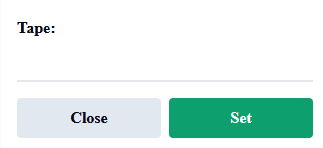
\includegraphics[width=0.4\textwidth]{Figures/PrntScrn_UI_TapeInput.png}
    \caption{Okno pro zadání vstupu}\label{fig:TapeInput}
\end{figure}

Samotný simulátor se pak skládá z několika částí. V horní částí je řádek, který symbolizuje vstupní pásku se symboly. Symbol s tmavším pozadím je symbol, který bude přečten jako další. Nalevo od něj jsou již přečtené symboly a napravo symboly ještě nepřečtené. Na pravé straně se pak nachází zásobník. Symbol, který se nachází nejvýše a má tmavší pozadí, je symbol na vrcholu zásobníku, takže bude přečten v dalším kroku. 

Na levé straně stránky se nachází tři oblasti seřazené ve sloupci. První oblast, která se nachází nejvýše, zobrazuje aktuální stav, ve kterém se nachází řídící jednotka. Ve druhé oblasti, která je na Obrázku~\ref{fig:Simulator} prázdná, se zobrazují možnosti volby dalšího přechodu u nedeterministických zásobníkových automatů. Příklad volby je na Obrázku~\ref{fig:TransitionFunctionChoosing}. Třetí část pak obsahuje ovládací prvky simulátoru. Tlačítko \texttt{Close simulation} ukončí simulaci a vrátí uživatele do hlavní nabídky.\ \texttt{Set new tape} otevře modální okno pro zadání vstupu, stejně jako při prvním otevření stránky.
Šipky pak slouží k samotnému ovládání simulace. Šipky na krajích slouží ke spuštění automatické simulace, šipky uvnitř pak slouží k manuálnímu krokování. Tlačítko uprostřed slouží k pozastavení simulace. Posledním ovládacím prvkem je posuvník, který slouží k nastavení času mezi jednotlivými kroky při automatické simulaci.

Poslední částí simulátoru je místo uprostřed obrazovky, které slouží k zobrazování informací. V horní částí jsou dvě tlačítka, které přepínají, co bude zrovna zobrazeno. Levé tlačítko slouží k zobrazení tabulky s definicí aktuálně používaného zásobníkového automatu, pravé pak slouží k~zobrazení historie přechodů již použitých v této simulaci.

\begin{figure}[h]
    \centering
    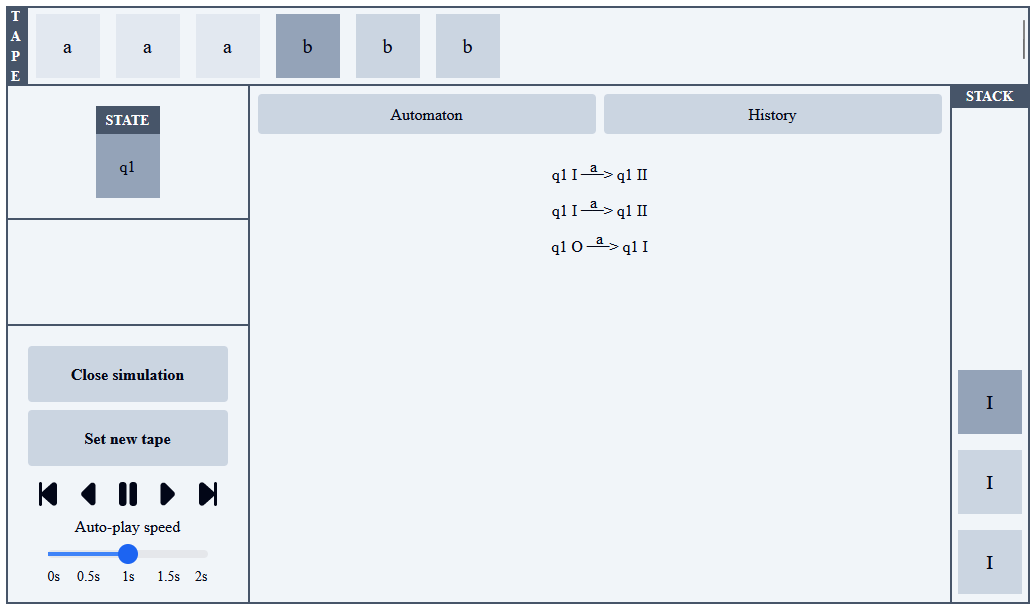
\includegraphics[width=\textwidth]{Figures/PrntScrn_UI_Simulator.png}
    \caption{Okno pro zadání vstupu}\label{fig:Simulator}
\end{figure}

\endinput